%
% body.tex
%
% Copyright © 2020 Libao Jin <jinlibao@outlook.com>
% Distributed under terms of the MIT license.
%
Please note that the deadline will be enforced as per the previous homework. Remember that you are allowed to work in teams of two on this assignment. You are encouraged to prepare your work in \LaTeX{}; a template will be provided to help you put it all together. If you choose  to submit a hard copy, you may submit only one copy for a team, indicating the names of both contributors. Online submission is encouraged, however, in that case both members of a team should submit the PDF file containing  their work and showing both their names. \\[20pt]
\textbf{Instruction}
\begin{enumerate}[label={\arabic*.}]
  \item Go to \url{https://www.overleaf.com} and sign in (required).
  \item Open \href{https://www.overleaf.com/read/qczrkwtzpxft}{template}, click \emph{Menu} (up left corner), then \emph{Copy Project}.
  \item Go to \verb|LaTeX/meta.tex| (the file \verb|meta.tex| under the folder \verb|LaTeX|) to change the section and your name, e.g.,
    \begin{itemize}
      \item change title to \verb|\title{MATH 3340-01 Scientific Computing Homework 3}|
      \item change author to \verb|\author{Albert Einstein \& Carl F. Gauss}|
    \end{itemize}
  \item For Problem 1, 2, 3, you need to write function/script files, store results to output files, and save graphs to figure files. Here are suggested names for function files, script files, output files, and figure files:
    \begin{table}[!hbtp]
      \centering
      % \caption{caption}
      % \label{tab:label}
      \begin{tabular}{cllll}
        \toprule
        Problem & Function File        & Script File     & Output File       & Figure File       \\
        \midrule
        1       & \verb|jacobi.m|      & \verb|hw3_p1.m| & \verb|hw3_p1.txt| & \verb|hw3_p1.pdf| \\
        2       & \verb|gaussSeidel.m| & \verb|hw3_p2.m| & \verb|hw3_p2.txt| & \verb|hw3_p2.pdf| \\
        3       &                      & \verb|hw3_p3.m| & \verb|hw3_p3.txt| & \verb|hw3_p3.pdf| \\
        \bottomrule
      \end{tabular}
    \end{table}

    Once finished, you need to upload these files to the folder \verb|src| on Overleaf. If you have different filenames, please update the filenames in \verb|\lstinputlisting{../src/your_script_name.m}| accordingly. You can code in the provided files in \href{https://libaoj.in/courses/2021s/MATH3340/Homework/3/hw3.zip}{hw3.zip}, and use the MATLAB script \verb|save_results.m| to generate the output files and store the graphs to \verb|.pdf| files automatically (the script filenames should be exactly same as listed above).
  \item Recompile, download, and submit the generated PDF.
  \item You may find \href{https://libaoj.in/files/LaTeX.Mathematical.Symbols.pdf}{\LaTeX{}.Mathematical.Symbols.pdf} and the second part of \href{https://libaoj.in/courses/2021s/MATH3341/slides/Math.3341.Lab.01.Slides.pdf}{Lab 01 Slides} and \href{https://libaoj.in/courses/2021s/MATH3341/slides/Math.3341.Lab.02.Slides.pdf}{Lab 02 Slides} helpful.
\end{enumerate}

\newpage
%%%%%%%%%%%%%%%%%%%%%%%%%%%%%%%%%%%%%%%%%%%%%%%%
% Problem 1
%%%%%%%%%%%%%%%%%%%%%%%%%%%%%%%%%%%%%%%%%%%%%%%%
\section{Problem 1}%
\label{sec:problem_1}
Solve, using a MATLAB code, the following system:
\begin{equation*}
  \begin{cases}
    5x - y + z + w   = 9 \\
    x + 7y + 2z + 2w = 3 \\
    2x + y + 5z + w  = 7 \\
    x - y + z + 4w   = 6
  \end{cases}
\end{equation*}
Use the Jacobi method with with a tolerance of $10^{-5}$ for the norm of the residual. Arrange your results in a table of the form
\begin{table}[!hbtp]
  \centering
  \caption{caption}
  \label{tab:label}
  \begin{tabular}{ccccc}
    \toprule
    iteration & $x$      & $y$      & $z$      & $w$      \\
    \midrule
    $0$       & $0$      & $0$      & $0$      & $0$      \\
    $1$       & $1$      & $2$      & $3$      & $4$      \\
    $\vdots$  & $\vdots$ & $\vdots$ & $\vdots$ & $\vdots$ \\
    \bottomrule
  \end{tabular}
\end{table}
so that you can see how $x$, $y$, $z$ and $w$ change with each iteration. You can create such a table using \verb|disp| in a loop; you may also use variants of \verb|printf| (in C Language), i.e., \verb|fprintf| or \verb|sprintf| if you are familiar with these functions, but do not use the MATLAB \verb|table| command as it does not do quite what is expected here. Also, as obvious from the table above, start with the zero guess. Moreover, plot the norm of the residual versus the iteration number; use a logarithmic scale on the vertical axis (the residual axis). Turn in your code and the output as described. The code can be organized as:
\begin{enumerate}
  \item a function file that implements Jacobi's method; and
  \item a script that calls the function with with the appropriate inputs and processes the results.\end{enumerate}
Your plot should have a plot title, axes labels and a legend. Use the \verb|help plot| command and the class notes  to investigate the various options  available when plotting.
\begin{solution}
  \quad
  \begin{itemize}
    \item
      Function file \verb|jacobi.m|
      \lstinputlisting[style=MATLAB]{../src/jacobi.m}
    \item
      Script file \verb|hw3_p1.m|
      \lstinputlisting[style=MATLAB]{../src/hw3_p1.m}
    \item
      Output file \verb|hw3_p1.txt|
      \lstinputlisting[style=Plain]{../src/hw3_p1.txt}
      \begin{figure}[!hbtp]
        \centering
        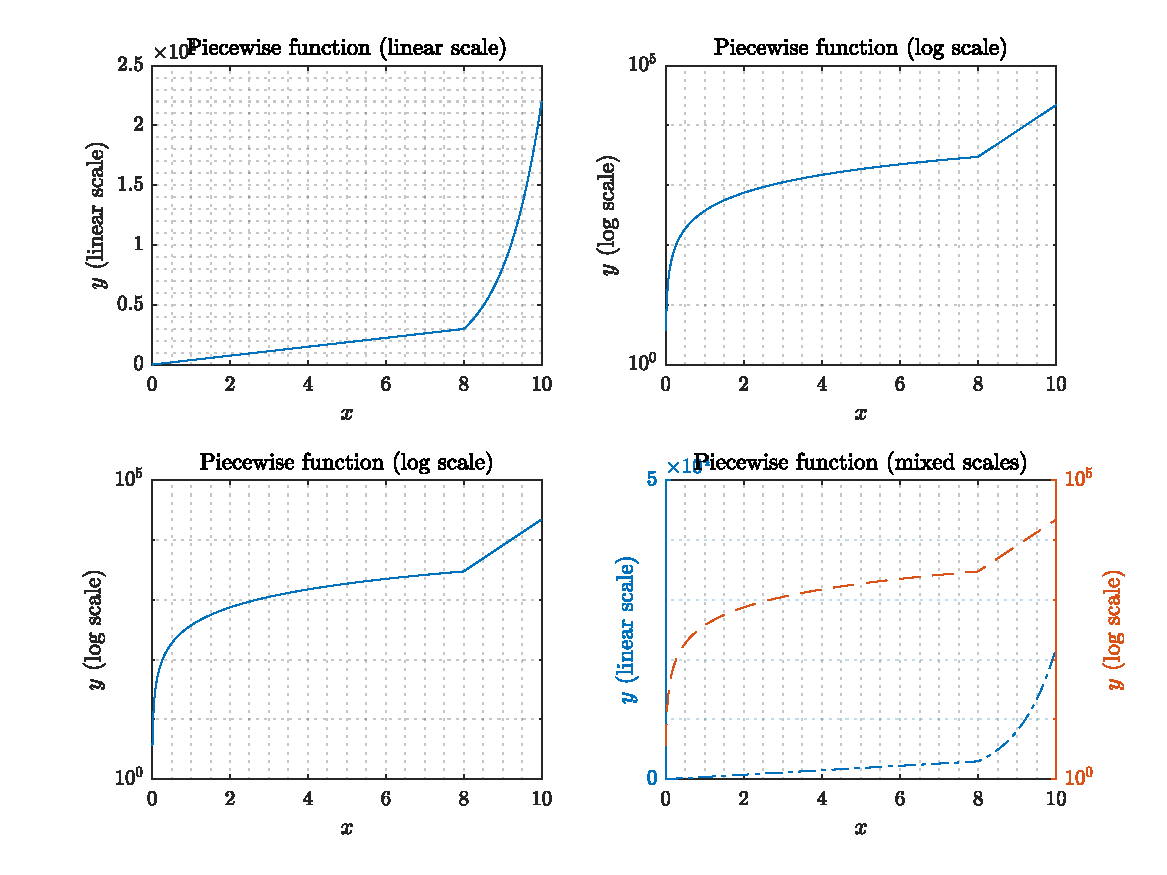
\includegraphics[width=0.8\linewidth]{../src/hw3_p1.pdf}
        \caption{}%
        \label{fig:}
      \end{figure}
  \end{itemize}
\end{solution}

%%%%%%%%%%%%%%%%%%%%%%%%%%%%%%%%%%%%%%%%%%%%%%%%
% Problem 2
%%%%%%%%%%%%%%%%%%%%%%%%%%%%%%%%%%%%%%%%%%%%%%%%
\section{Problem 2}%
\label{sec:problem_2}
Solve again the system above, in MATLAB, using the Gauss-Seidel method. Produce the same results as for the previous problem.
\begin{solution}
  \quad
  \begin{itemize}
    \item
      Function file \verb|gaussSeidel.m|
      \lstinputlisting[style=MATLAB]{../src/gaussSeidel.m}
    \item
      Script file \verb|hw3_p2.m|
      \lstinputlisting[style=MATLAB]{../src/hw3_p2.m}
    \item
      Output file \verb|hw3_p2.txt|
      \lstinputlisting[style=Plain]{../src/hw3_p2.txt}
      \begin{figure}[!hbtp]
        \centering
        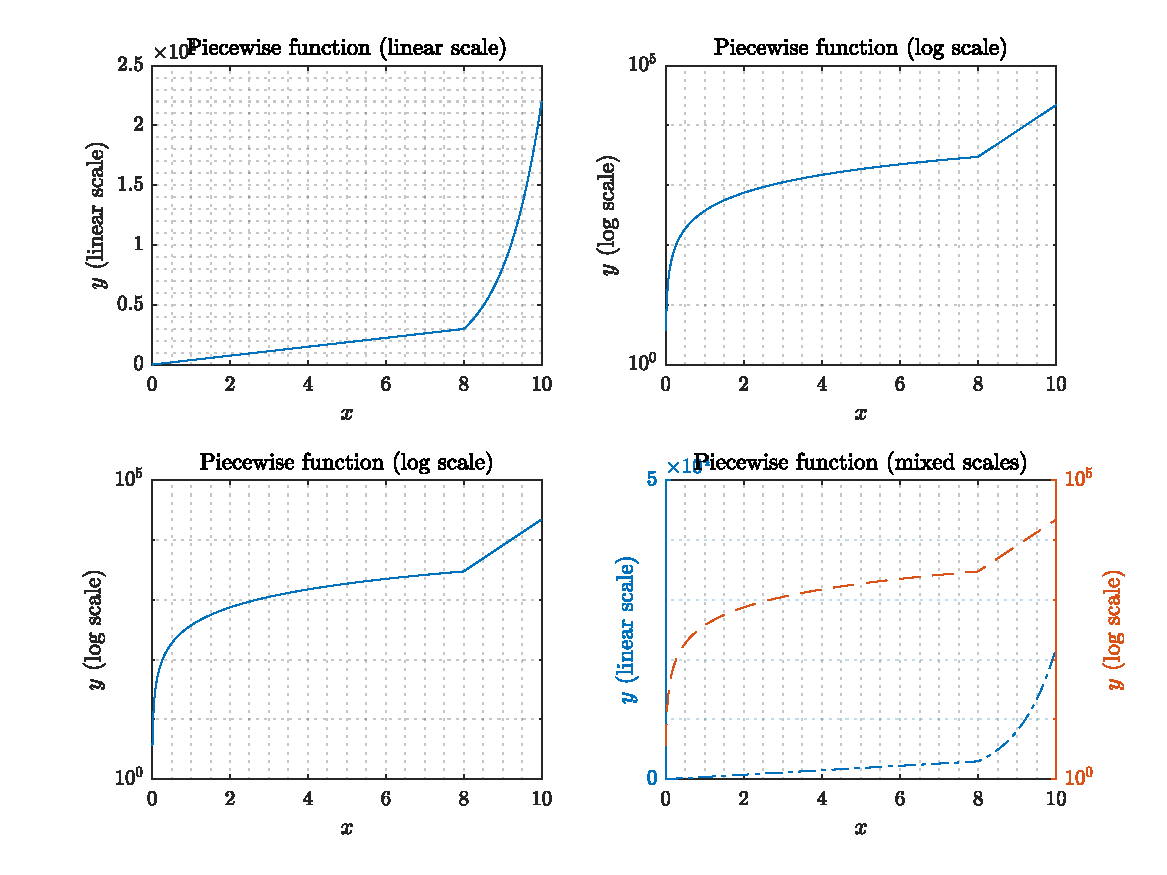
\includegraphics[width=0.8\linewidth]{../src/hw3_p2.pdf}
        \caption{}%
        \label{fig:}
      \end{figure}
  \end{itemize}
\end{solution}

%%%%%%%%%%%%%%%%%%%%%%%%%%%%%%%%%%%%%%%%%%%%%%%%
% Problem 3
%%%%%%%%%%%%%%%%%%%%%%%%%%%%%%%%%%%%%%%%%%%%%%%%
\section{Problem 3}%
\label{sec:problem_3}
Solve the twenty-one systems of equations:
\begin{equation*}
  \begin{cases}
    7x + y + 2z = 0.01 m^{2} - 2m \\
    x - 5y + 2z = 2 - m \\
    2x + y + 5z = 9
  \end{cases}
\end{equation*}
obtained by setting, in turn, the value of the quantity $m$ on the right-hand side to all integers in between, and including, $m = 0$ and $m = 20$. This time use the LU-decomposition of the system matrix that is implemented in MATLAB by the \verb|lu| function. Perform the decomposition only once, then use the lower- and upper-triangular factors repeatedly to find each successive solution. Turn in the code and a plot of the first and second components of the solution (that is, the values of $x$ and $y$) as a function of thee right-hand side parameter $m$.
\begin{solution}
  \quad
  \begin{itemize}
    \item
      Script file \verb|hw3_p3.m|
      \lstinputlisting[style=MATLAB]{../src/hw3_p3.m}
    \item
      Output file \verb|hw3_p3.txt|
      \lstinputlisting[style=Plain]{../src/hw3_p3.txt}
      \begin{figure}[!hbtp]
        \centering
        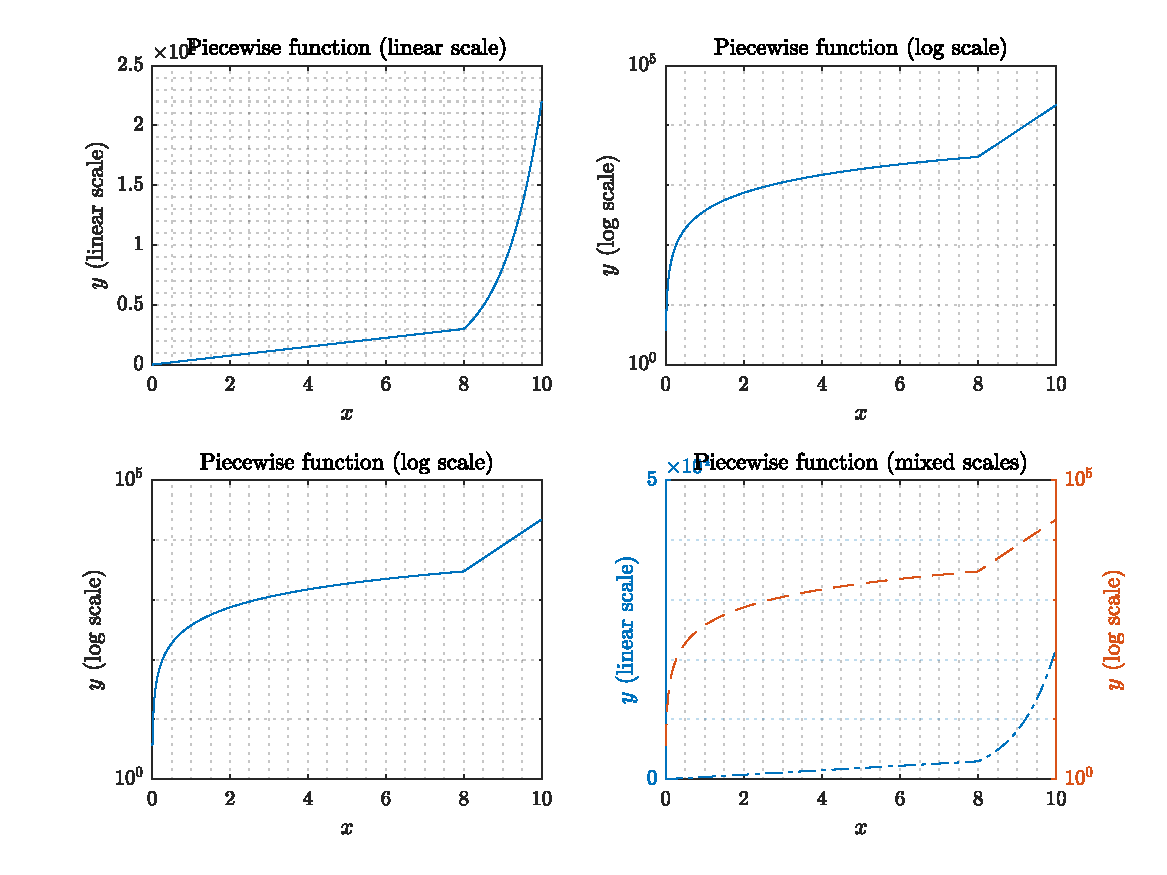
\includegraphics[width=0.8\linewidth]{../src/hw3_p3.pdf}
        \caption{}%
        \label{fig:}
      \end{figure}
  \end{itemize}
\end{solution}

